\chapter{Research}
\label{ch:background}

This chapter provides background context for the development of a liquid democracy system within Vodle. It builds on the concepts introduced earlier, focusing on more detailed research into known limitations of liquid democracy and potential solutions proposed in academic literature. Additionally, the technical foundations and design philosophy of Vodle as a platform are explored.

\section{Liquid Democracy}

Liquid democracy, or delegative voting, allows voters to either cast a vote directly, delegate it to someone they trust, or abstain \citep{blum_liquid_2016}. A key feature is that delegations are transitive - a chain of users that all delegate to each other sequentially ends with a single final voter who casts their vote on behalf of all those in the chain.

Whilst the transitivity property enables concentration of voting power with trusted individuals, it can also lead to unintended consequences. Chains of delegations may result in cycles that prevent votes from being cast, or allow certain individuals to accumulate an excessive share of influence, creating so-called super-voters. These problems amongst others motivate the need for alternative delegation mechanisms, as discussed in the following subsections.

%\cite{ford_delegative_2002} argues that direct democracy becomes ineffective at scale due to the diversity in participants' knowledge and interest. Without mechanisms to channel influence through trusted intermediaries, the collective outcome may reflect average rather than informed decision-making. Liquid democracy addresses this by enabling voters to shift influence toward participants with greater expertise or engagement.

\subsection{Issues with Liquid Democracy}

\subsubsection{Delegation cycles}
\begin{figure}[h]
    \centering
    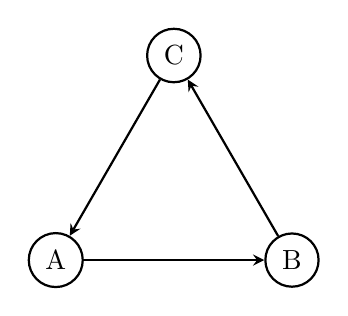
\begin{tikzpicture}[->, >=stealth, thick, scale=1.5]
        % Nodes at triangle vertices
        \node[circle, draw] (A) at (0,0) {A};
        \node[circle, draw] (B) at (2,0) {B};
        \node[circle, draw] (C) at (1,1.732) {C}; % height = sqrt(3)

        % Arrows showing delegation
        \draw (A) -- (B);
        \draw (B) -- (C);
        \draw (C) -- (A);
    \end{tikzpicture}
    \caption{Delegation cycle: A delegates to B, B to C, and C back to A.}
    \label{fig:triangle-cycle}
\end{figure}


Delegation cycles occur when a vote is delegated in such a way that it ends up forming a loop \citep{brill_liquid_2022}, preventing the vote from reaching a final, resolvable destination. For example, if Alice delegates her vote to Bob, Bob delegates to Charlie, and Charlie delegates back to Alice, the votes become trapped in a cycle (seen above) and can be treated as a loss of representation \citep{christoff2017liquiddemocracyanalysisbinary}.

This issue is particularly problematic because it can nullify votes without the affected users ever realising. In systems where cycles are not explicitly detected and handled, these votes are discarded silently, potentially changing the final outcome of the votes.

Delegation cycles are increasingly likely to emerge in dynamic voting systems, where delegations can be added, removed, or modified at any point in time. Delegations that initially did not form part of a cycle may later contribute to one as other voters add a new delegation or alter an existing one.

\textit{Paragraph on how size of the system affects the possibility of cycles?}

\subsubsection{Abstentions}
\begin{figure}[h]
    \centering
    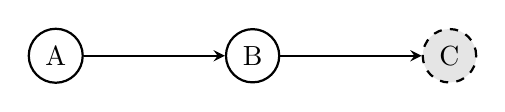
\begin{tikzpicture}[->, >=stealth, thick, node distance=2.5cm]
        \node[circle, draw] (A) {A};
        \node[circle, draw, right of=A] (B) {B};
        \node[circle, draw, right of=B, dashed, fill=gray!20] (C) {C};

        \draw (A) -- (B);
        \draw (B) -- (C);
    \end{tikzpicture}
    \caption{Delegation chain ending in abstention: A delegates to B, B to C. C abstains, causing the votes of A and B to be lost.}
    \label{fig:delegation-abstention}
\end{figure}

In liquid democracy, abstention is where a voter neither casts a vote nor delegates their vote to another user \citep{brill_liquid_2022}. This includes both deliberate abstention, where a voter knowingly chooses not to participate, and passive abstention, where a voter may be unaware of an ongoing poll or are unable to engage with it.

Abstentions are especially impactful when they occur at the end of a larger delegation chain, as all votes passed along the chain to that voter are effectively lost \citep{brill_liquid_2022}. The voters whose decisions were passed along the chain may also be unaware that their votes have been nullified, worsening the effect of the abstention.

\subsubsection{Super-voters}
In liquid democracy, a super-voter is an individual who receives a large number of delegated votes, therefore gaining disproportionate influence over decisions \citep{kling2015votingbehaviourpoweronline}. While this behaviour may reflect voters' genuine preferences, it can lead to a concentration of power that goes against the intended egalitarianism and democratic ideals of liquid democracy.

Although liquid democracy allows users to alter their delegation at any time, in practice, many voters may not actively monitor or even know how their vote is being used. This can allow a small number of super-voters to dominate outcomes, especially in systems with large delegation chains.

Real-world examples of this phenomenon have been documented. In the German Pirate Party's use of LiquidFeedback, certain users received so many delegations that their votes were like "decrees" \citep{sven_becker_liquid_2012,kling2015votingbehaviourpoweronline} even though they were not elected officials. \cite{kling2015votingbehaviourpoweronline} noted that the super-voters generally voted in line with the majority, therefore not drastically affecting the outcome of the votes and contributed to the stability of the system. However, the potential for individuals to single-handedly influence the results remained a concern.
%This pattern has also been observed in blockchain-based governance systems \citep{hallWhatHappensWhen2024}, where voting tokens (digital representations of voting power) are commonly concentrated among a few delegates, giving them an excessive amount of power.
%In the case of the Pirate Party, analysis showed that although super-voters held significant theoretical power, they generally voted in line with the majority, therefore not drastically affecting the outcome of the votes. \cite{kling2015votingbehaviourpoweronline} described this behaviour as voting "wisely," noting that while these individuals had the capacity to change outcomes, they typically did not use it to push their own agenda.

This pattern is not limited to traditional online voting platforms. It can also be seen within decentralised autonomous organisations (DAOs) - blockchain-based entities where decisions are made collectively by token holders without central leadership. These organisations use token-based voting to decide on critical issues like protocol upgrades and funding allocations. \cite{hallWhatHappensWhen2024} studied 18 decentralised autonomous organisations (DAOs) and found that voting power was often concentrated in the hands of a few delegates. While most did not control a large share of all available tokens, low participation meant that their share of actual votes cast was disproportionately high. In several DAOs, the top five delegates accounted for over 50\% of all votes cast, and in the DAO Gitcoin, this figure exceeded 90\%.
\subsection{Variations of Liquid Democracy}

\subsubsection{Ranked delegation} Allows voters to specify fall-back delegates in order of preference (Brill et al., 2022).

Include different algorithms from Brill paper

\subsubsection{Weighted/ vote splitting}
Voting power is distributed across multiple delegates to reduce reliance on any single individual (\cite{golz_fluid_2021}).

\subsubsection{Backup votes - kinda unneeded}
Voters may provide a direct vote to use in case delegation fails.

\section{Implementations of Liquid Democracy}
\subsection{LiquidFeedback}
\subsection{Google Votes}

\section{vodle}
Vodle is a web-based platform for participatory group decision-making. Users participate in polls that allow them to rate a set of options using sliders. These sliders enable users to express degrees of preference rather than make binary choices. The platform aggregates these ratings to derive results that reflect the collective input of the voters in each poll.

\subsection{MaxParC}

\textbf{Maximal Participation and Consensus (MaxParC)}: A proportional decision-making method that encourages widespread involvement and compromise.

\textbf{Conditional commitments}: Voters can condition their support based on how others are expected to vote, supporting consensus-building.

\textbf{Role in Vodle}: MaxParC is used as the primary aggregation mechanism within Vodle.

\subsection{Architecture}

\textbf{Client-server model}: Facilitates real-time voting through a web interface.

\textbf{Poll-based interaction}: Users rate options in predefined polls.

\textbf{Extensibility}: The platform's architecture supports the integration of new decision-making models, such as liquid democracy.

\subsection{Design Philosophy}

\textbf{Minimalism}: Designed to reduce friction and make participation intuitive.

\textbf{Flexibility}: Supports a range of decision models.

\textbf{Legibility}: Users can understand and trust how results are derived.

\section{Summary}
This chapter reviewed the structure and challenges of liquid democracy, explored enhancements found in recent literature, and outlined Vodle's technical and conceptual foundation. These insights inform the design and implementation decisions discussed in the next chapters.

